\textbf{COLUNI 2026 -- Questão 12}\par\medskip Muitos estabelecimentos comerciais oferecem para seus clientes internet gratuita (Wi-fi). Geralmente, para ter-se acesso a esse benefício, basta perguntar a algum funcionário do estabelecimento o “login” e a “senha” do Wi-fi.

O dono da pizzaria “Boa $\pi$tiza” resolveu inovar e, ao invés de fornecer os dados para o acesso ao Wi-fi, pregou o seguinte cartaz na parede de sua pizzaria:

% COLUNI-AUTO-FIGURES-BEGIN
\begin{figure}[htbp]
\centering
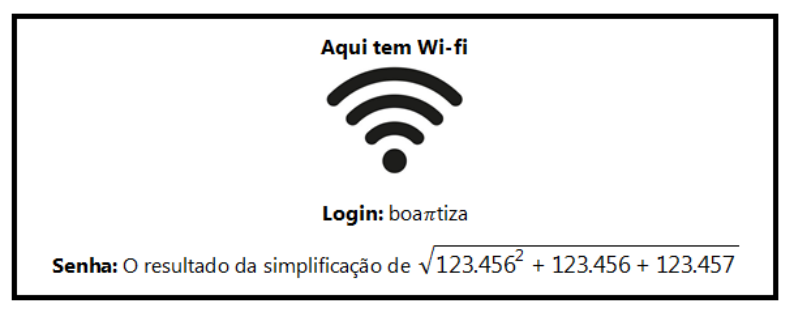
\includegraphics[width=0.8\linewidth]{static/simulados/coluni/figuras/2026/questao-12/figura-1.png}
\end{figure}
% COLUNI-AUTO-FIGURES-END

É CORRETO afirmar que a senha indicada no cartaz é:
\begin{enumerate}
\item 123.456
\item $123.456^2$
\item 123.457
\item $123.457^2$
\end{enumerate}
